While direct attacks on the latter are possible, in this work, we
take a language-agnostic approach to improving Recurrent Neural
Networks (RNN, \cite{rumelhart1988learning}), which brought about many
advances in tasks such as language modelling, semantic parsing,
machine translation, with no shortage of non-NLP applications either
\citep{bakker2002reinforcement,mayer2008system}.
%
Many neural models are built from RNNs including the
sequence-to-sequence family \citep{sutskever2014sequence} and its
attention-based branch \citep{bahdanau2014neural}.
%
Thus, innovations in RNN architecture tend to have a trickle-down
effect from language modelling, where evaluation is often the easiest
and data the most readily available, to many other tasks, a trend
greatly strengthened by ULMFiT \citep{howard2018universal}, ELMo
\citep{peters2018deep} and BERT \citep{devlin2018bert}, which promote
language models from architectural blueprints to pretrained building
blocks.

To improve the generalization ability of language models, we propose
an extension to the LSTM \citep{hochreiter1997lstm}, where the LSTM's
input $\vx$ is gated conditioned on the output of the previous step
$\vhprev$.
%
Next, the gated input is used in a similar manner to gate the output
of the previous time step.
%
After a couple of rounds of this mutual gating, the last updated $\vx$
and $\vhprev$ are fed to an LSTM.
%
With the addition of more gating, in one sense,
our model joins the long list of recurrent architectures with gating
structures of varying complexity that followed the invention of Elman
Networks \citep{elman1990finding}.
%
Examples include the LSTM, the GRU \citep{chung2015gated}, and even
designs by Neural Architecture Search
\citep{DBLP:journals/corr/ZophL16}.

Intuitively, in the lowermost layer, the first gating step scales the
input embedding (itself a representation of the \emph{average} context
in which the token occurs) depending on the \emph{actual} context,
resulting in a contextualized representation of the input.
%
While intuitive, as \Cref{sec:mog-analysis} shows, this
interpretation cannot account for all the observed phenomena.

In a more encompassing view, our model can be seen as enriching the
mostly additive dynamics of recurrent transitions placing it in the
company of the Input Switched Affine Network \citep{foerster2017input}
with a separate transition matrix for each possible input, and the
Multiplicative RNN \citep{sutskever2011generating}, which factorizes
the three-way tensor of stacked transition matrices.
%
Also following this line of research are the Multiplicative
Integration LSTM \citep{wu2016multiplicative} and --~closest to our
model in the literature~-- the Multiplicative LSTM
\citep{DBLP:journals/corr/KrauseLMR16}.
%
The results in \Cref{sec:results} demonstrate the utility of
our approach, which consistently improves on the LSTM and establishes
a new state of the art on all but the largest dataset, \enwik, where
we match similarly sized transformer models.

\section{Model}

To allow for ease of subsequent extension, we present the standard
LSTM update \citep{DBLP:journals/corr/SakSB14} with input and state of
size $m$ and $n$ respectively as the following function:
\begin{gather*}
\LSTM \colon \Rb^n\times\Rb^n \times \Rb^m \to \Rb^n \times \Rb^n \\
\LSTM\bigl(\vcprev, \vhprev, \vx\bigr) = \bigl(\vc, \vh\bigr).
\end{gather*}
%
The updated state $\vc$ and the output $\vh$ are computed as follows:
\begin{equation}
\label{eq:lstm}
\begin{aligned}
  \vf &= \sigma\bigl(\mW^{fx} \vx + \mW^{fh} \vhprev + \vb^f\bigr) \\
  \vi &= \sigma\bigl(\mW^{ix} \vx + \mW^{ih} \vhprev + \vb^i\bigr) \\
  \vj &= \tanh\bigl(\mW^{jx}\vx + \mW^{jh} \vhprev + \vb^j\bigr) \\
  \vo &= \sigma\bigl(\mW^{ox} \vx + \mW^{oh} \vhprev + \vb^o\bigr) \\
  \vc &= \vf \odot \vcprev + \vi \odot \vj \\
  \vh &= \vo \odot \tanh\bigl(\vc\bigr),
\end{aligned}
\end{equation}
where $\sigma$ is the logistic sigmoid function, $\odot$ is the
elementwise product, $\mW^{**}$ and $\vb^{*}$ are weight matrices and
biases.

\begin{figure}[!t]\centering
  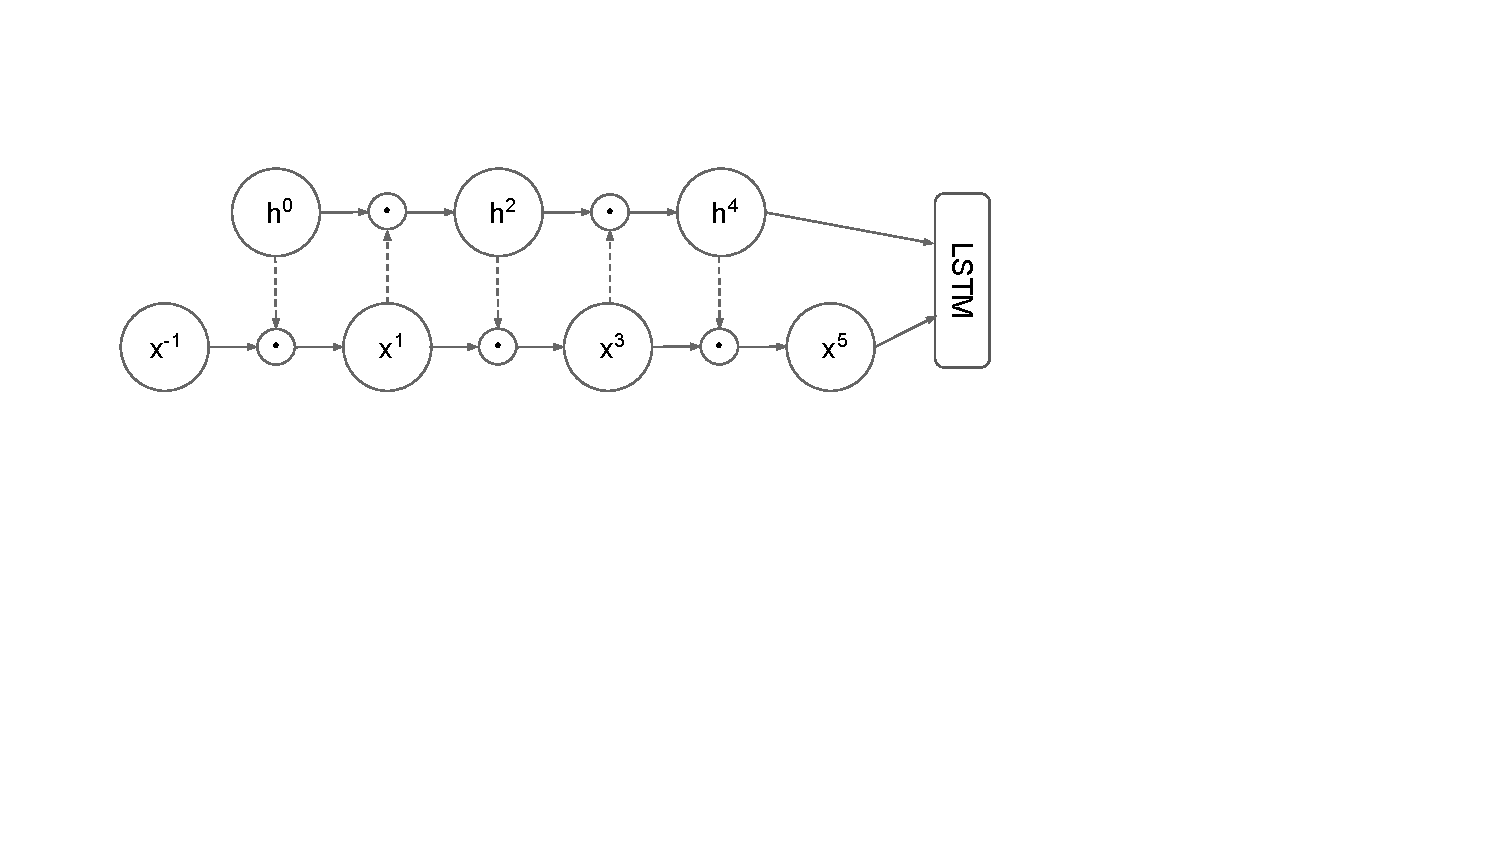
\includegraphics[scale=0.7,trim={1.8cm 7.5cm 8.3cm 2.5cm},clip]
                  {mogrifier/figure/mogrifier.pdf}
  \caption[Mogrifier with 5 rounds of updates.]{Mogrifier with
    5 rounds of updates. The previous state $\vh^0=\vhprev$ is
    transformed linearly (dashed arrows), fed through a sigmoid and
    gates $\vx^{-1}=\vx$ in an elementwise manner producing $\vx^1$.
    Conversely, the linearly transformed $\vx^1$ gates $\vh^0$ and
    produces $\vh^2$. After a number of repetitions of this mutual
    gating cycle, the last values of $\vh^*$ and $\vx^*$ sequences are
    fed to an LSTM cell. The \emph{prev} subscript of $\vh$ is omitted
    to reduce clutter.}
  \label{fig:mogrifier}
\end{figure}
%
While the LSTM is typically presented as a solution to the vanishing
gradients problem, its gate $i$ can also be interpreted as scaling the
rows of weight matrices $\mW^{j*}$ (ignoring the non-linearity in
$j$).
%
In this sense, the LSTM nudges Elman Networks towards
context-dependent transitions and the extreme case of Input Switched
Affine Networks.
%
If we took another, larger step towards that extreme, we could end up
with Hypernetworks \citep{ha2016hypernetworks}.
%
Here, instead, we take a more cautious step and equip the LSTM with
gates that scale the \emph{columns} of all its weight matrices
$\mW^{**}$ in a context-dependent manner.
%
The scaling of the matrices $\mW^{*x}$ (those that transform the cell
input) makes the input embeddings dependent on the cell state, while
the scaling of $\mW^{*h}$ does the reverse.

As \Cref{fig:mogrifier} illustrates, the Mogrifier\footnote{It's like
a transmogrifier\footnotemark{} without the magic: it can only shrink
or expand objects.}\footnotetext{Transmogrify (verb, 1650s): to
completely alter the form of something in a surprising or magical
manner.}
LSTM is an LSTM where two inputs $\vhprev$ and $\vx$ modulate
one another in an alternating fashion before the usual LSTM
computation takes place.
That is,
\begin{gather*}
\mathrm{MogrifierLSTM} \colon \Rb^n\times\Rb^n \times \Rb^m \to \Rb^n \times \Rb^n \\
\LSTM\bigl(\vcprev, \mogrify(\vhprev, \vx)\bigr) = \bigl(\vc, \vh\bigr),
\end{gather*}
where the mogrification operation is the following $\Rb^n\times\Rb^m \to \Rb^n \times \Rb^m$ function:
{\def\groundprop{1.5}
\begin{equation}
\label{eq:mogrify}
\begin{aligned}
  \mogrify(\vh,\vx) &= \vh^{2\floor{r/2}}, \vx^{2\floor{(r+1)/2}-1}\\
  \vx^{-1}, \vh^0 &= \vx, \vh\\
  \vx^i &= 2\sigma\bigl(\mQ^{i}\vh^{i-1}\bigr) \odot \vx^{i-2} &
  \text{for odd i} \in [1..r],\\
  \vh^i &= 2\sigma\bigl(\mR^{i}\vx^{i-1}\bigr) \odot \vh^{i-2}
  & \text{for even i} \in [1..r].
\end{aligned}
\end{equation}}%
Here, the number of rounds, $r \in \Nb$, is a hyperparameter;
$r=0$ recovers the identity function.
%
Multiplication with the constant $2$ ensures that randomly initialized
$\mQ^{i}, \mR^{i}$ matrices result in transformations close to
identity.
%
To reduce the number of additional model parameters, we typically
factorize the $\mQ^{i}, \mR^{i}$ matrices as products of low-rank
matrices: $\mQ^i = \mQ^i_{\textrm{left}} \mQ^i_{\textrm{right}}$ with
$\mQ^i \in \Rb^{m \times n}, \mQ^i_{\textrm{left}} \in
\Rb^{m \times k}, \mQ^i_{\textrm{right}} \in \Rb^{k
  \times n}$, where $k<min(m,n)$ is the rank.\\[-\groundskip]

\section{Experiments}

\subsection{Datasets}

We compare models on both word and character-level language modelling
datasets.
%
The two word-level datasets we picked are the Penn Treebank (\ptb)
corpus by \citet{marcus1993building} with preprocessing from
\citet{mikolov2010recurrent} and \wikitexttwo by
\citet{DBLP:journals/corr/MerityXBS16}, which is about twice the size
of \ptb with a larger vocabulary and lighter preprocessing.
%
These datasets are definitely on the small side, but --~and
\emph{because} of this~-- they are suitable for exploring different
model biases.
%
Their main shortcoming is the small vocabulary size, only in the tens
of thousands, which makes them inappropriate for exploring the
behaviour of the long tail.
%
For that, open vocabulary language modelling and byte pair encoding
\citep{sennrich2015neural} would be an obvious choice.
%
Still, our primary goal here is the comparison of the LSTM and
Mogrifier architectures, thus we instead opt for character-based
language modelling tasks, where vocabulary size is not an issue, the
long tail is not truncated, and there are no additional
hyperparameters as in byte pair encoding that make fair comparison
harder.
%
The first character-based corpus is \enwik from the Hutter Prize
dataset \citep{hutter2012human}.
%
Following common practice, we use the first 90 million characters for
training and the remaining 10 million evenly split between validation
and test.
%
The character-level task on the Mikolov preprocessed \ptb corpus
\citep{merity2018analysis} is unique in that it has the disadvantages
of closed vocabulary without the advantages of word-level modelling,
but we include it for comparison to previous work.
%
The final character-level dataset is the Multilingual Wikipedia Corpus
(MWC, \cite{kawakami2017learning}), from which we focus on the English
and Finnish language subdatasets in the single text, large setting.

\begin{table}[t]
  \caption[Word-level perplexities of near state-of-the-art
    models.]{Word-level perplexities of near state-of-the-art
    models, our LSTM baseline and the Mogrifier on
    \ptb and \wikitexttwo. Models with Mixture of Softmaxes
    \citep{yang2017breaking} are denoted with \emph{MoS}, depth N with
    \emph{dN}. \emph{MC} stands for Monte Carlo dropout evaluation.
    Previous state-of-the-art results in italics. Note the comfortable
    margin of 2.8--4.3 perplexity points the Mogrifier enjoys over the
    LSTM.}
  \label{tab:mog-word-results}
  \small
  \centering
  \begin{tabular}{@{}llrlrlr@{}}
    & & & \multicolumn{2}{c}{No Dyneval} & \multicolumn{2}{c}{Dyneval} \\
    \cmidrule(lr){4-5} \cmidrule(l){6-7}
    & & & Val. & Test & Val. & Test \\
    \midrule
    \parbox[t]{2mm}{\multirow{7}{*}{\rotatebox[origin=c]{90}{PTB}}}
    & FRAGE (d3, MoS15) \citep{gong2018frage} & 22M
        & \emph{54.1} & \emph{52.4} & \emph{47.4} & \emph{46.5} \\
    & AWD-LSTM (d3, MoS15) \citep{yang2017breaking} & 22M
        & 56.5 & 54.4 & 48.3 & 47.7 \\
    & Transformer-XL \citep{dai2019transformer} & 24M
        & 56.7 & 54.5 & & \\
    & \textbf{LSTM} (d2) & 24M
        & \nlltoppl{4.02163} & \nlltoppl{3.99985}
        & \nlltoppl{3.88947} & \nlltoppl{3.88038} \\
    & \textbf{Mogrifier} (d2) & 24M
        & \nlltoppl{3.95346} & \nlltoppl{3.93124}
        & \nlltoppl{3.80963} & \nlltoppl{3.80708} \\
    & \textbf{LSTM} (d2, MC) & 24M
        & \nlltoppl{4.01559} & \nlltoppl{3.99003}
        & \nlltoppl{3.88338} & \nlltoppl{3.87987} \\
    & \textbf{Mogrifier} (d2, MC) & 24M
        & \nlltopplbold{3.93959} & \nlltopplbold{3.91415}
        & \nlltopplbold{3.80420} & \nlltopplbold{3.80321} \\
    \midrule
    \parbox[t]{2mm}{\multirow{6}{*}{\rotatebox[origin=c]{90}{WT$2$}}}
    & FRAGE (d3, MoS15) \citep{gong2018frage} & 35M
        & \emph{60.3} & \emph{58.0} & \emph{40.8} & \emph{39.1} \\
    & AWD-LSTM (d3, MoS15) \citep{yang2017breaking} & 35M
        & 63.9 & 61.2 & 42.4 & 40.7 \\
    & \textbf{LSTM} (d2, MoS2) & 35M
        & \nlltoppl{4.13609} & \nlltoppl{4.09557}
        & \nlltoppl{3.76661} & \nlltoppl{3.72658} \\
    & \textbf{Mogrifier} (d2, MoS2) & 35M
        & \nlltoppl{4.07235} & \nlltoppl{4.03665}
        & \nlltoppl{3.70429} & \nlltoppl{3.66475} \\
    & \textbf{LSTM} (d2, MoS2, MC) & 35M
        & \nlltoppl{4.12526} & \nlltoppl{4.08426}
        & \nlltoppl{3.76540} & \nlltoppl{3.72385} \\
    & \textbf{Mogrifier} (d2, MoS2, MC) & 35M
        & \nlltopplbold{4.04771} & \nlltopplbold{4.00976}
        & \nlltopplbold{3.69399} & \nlltopplbold{3.65337} \\
    \midrule
  \end{tabular}
\end{table}

\subsection{Setup}

We tune hyperparameters following the experimental setup of
\cite{melis2018pushing} using a black-box hyperparameter tuner based
on batched Gaussian Process Bandits \citep{golovin2017google}.
%
For the LSTM, the tuned hyperparameters are the same:
\emph{input\_embedding\_ratio}, \emph{learning\_rate},
\emph{l2\_penalty}, \emph{input\_dropout},
\emph{inter\_layer\_dropout}, \emph{state\_dropout},
\emph{output\_dropout}.
%
For the Mogrifier, the number of rounds $r$ and the rank $k$ of the
low-rank approximation is also tuned (allowing for full rank, too).
%
For word-level tasks, BPTT \citep{werbos1990backpropagation} window
size is set to 70 and batch size to 64.
%
For character-level tasks, BPTT window size is set to 150 and batch
size to 128 except for \enwik where the window size is 500.
%
Input and output embeddings are tied for word-level tasks following
\cite{DBLP:journals/corr/InanKS16} and
\cite{DBLP:journals/corr/PressW16}.
%
Optimization is performed with Adam \citep{kingma2014adam} with
$\beta_1=0$, a setting that resembles RMSProp without momentum.
%
Gradients are clipped \citep{pascanu2013difficulty} to norm 10.
%
We switch to averaging weights similarly to
\cite{merity2017regularizing} after a certain number of checkpoints
with no improvement in validation cross-entropy or at 80\% of the
training time at the latest.
%
We found no benefit to using two-step finetuning.

Model evaluation is performed with the standard, deterministic dropout
approximation or Monte Carlo averaging \citep{gal2016theoretically}
where explicitly noted (MC).
%
In standard dropout evaluation, dropout is turned off while in MC
dropout predictions are averaged over randomly sampled dropout masks
(200 in our experiments).
%
Optimal softmax temperature is determined on the validation set, and
in the MC case, dropout rates are scaled \citep{melis2018pushing}.
%
Finally, we report results with and without dynamic evaluation
\citep{krause2017dynamic}.
%
Hyperparameters for dynamic evaluation are tuned using the same method
(see \Cref{sec:hyperparameter-tuning-ranges} for details).

%% We make the code and the tuner output available at
%% \href{https://github.com/deepmind/lamb}{https://github.com/deepmind/lamb}.

\begin{table}[t!]
  \caption[Bits per character on character-based datasets of near
    state-of-the-art models.]{Bits per character on
    character-based datasets of near state-of-the-art models, our
    LSTM baseline and the Mogrifier. Previous
    state-of-the-art results in italics. Depth N is denoted with
    \emph{dN}. MC stands for Monte Carlo dropout evaluation. Once
    again the Mogrifier strictly dominates the LSTM and sets a new
    state of the art on all but the \enwik dataset where with dynamic
    evaluation it closes the gap to the Transformer-XL of similar size
    ($\dag$ \cite{krause2019dynamic}, $\ddag$ Ben Krause, personal
    communications, May 17, 2019). On most datasets, model size was
    set large enough for underfitting not to be an issue. This was
    very much not the case with \enwik, so we grouped models of
    similar sizes together for ease of comparison. Unfortunately, a
    couple of dynamic evaluation test runs diverged (NaN) on the test
    set and some were just too expensive to run (\enwik, MC).}
  \label{tab:mog-character-results}
  \centering
  \small
  \begin{tabular}{@{}llrllll@{}}
    & & & \multicolumn{2}{c}{No Dyneval} & \multicolumn{2}{c}{Dyneval} \\
    \cmidrule(lr){4-5} \cmidrule(lr){6-7}
    & & & Val. & \multicolumn{1}{r}{Test} & Val. & \multicolumn{1}{r}{Test} \\
    \midrule
    \parbox[t]{2mm}{\multirow{6}{*}{\rotatebox[origin=c]{90}{PTB}}}
    & Trellis Networks \citep{bai2018trellis} & 13.8M & & \emph{1.159} & & \\
    & AWD-LSTM (d3) \citep{merity2017regularizing} & 13.8M & & 1.175 & & \\
    & \textbf{LSTM} (d2) & 24M
        & \nlltobpc{0.80641} & \nlltobpc{0.79259}
        & \nlltobpc{0.77349} & \nlltobpc{0.76448} \\
    & \textbf{Mogrifier} (d2) & 24M
        & \nlltobpc{0.79616} & \nlltobpc{0.78415}
        & \nlltobpc{0.76119} & \nlltobpc{0.75439} \\
    & \textbf{LSTM} (d2, MC) & 24M
        & \nlltobpc{0.80331} & \nlltobpc{0.78936}
        & \nlltobpc{0.77262} & \nlltobpc{0.76353} \\
    & \textbf{Mogrifier} (d2, MC) & 24M
        & \nlltobpcbold{0.78829} & \nlltobpcbold{0.77642}
        & \nlltobpcbold{0.75861} & \nlltobpcbold{0.75069} \\
    \midrule
    \multirow{6}{*}{\rotatebox[origin=c]{90}{MWC\,\, EN}}
    & HCLM+Cache \citep{kawakami2017learning} & 8M
        & \emph{1.591} & \emph{1.538} & & \\
    & LSTM (d1) \citep{kawakami2017learning} & 8M
        & 1.793 & 1.736 & & \\
    & \textbf{LSTM} (d2) & 24M
        & \nlltobpc{0.93766} & \nlltobpc{0.92752}
        & \nlltobpc{0.85915} & \nlltobpc{0.84918} \\
    & \textbf{Mogrifier} (d2) & 24M
        & \nlltobpc{0.91464} & \nlltobpc{0.90439}
        & \nlltobpc{0.83346} & \nlltobpc{0.82386} \\
    & \textbf{LSTM} (d2, MC) & 24M
        & \nlltobpc{0.93336} & \nlltobpc{0.92356}
        & \nlltobpc{0.85783} & NaN \\
    & \textbf{Mogrifier} (d2, MC) & 24M
        & \nlltobpcbold{0.90977} & \nlltobpcbold{0.89980}
        & \nlltobpcbold{0.83193} & \nlltobpcbold{0.82302} \\
    \midrule
    \multirow{6}{*}{\rotatebox[origin=c]{90}{MWC\,\, FI}}
    & HCLM+Cache \citep{kawakami2017learning} & 8M
        & \emph{1.754} & \emph{1.711} & & \\
    & LSTM (d1) \citep{kawakami2017learning} & 8M
        & 1.943 & 1.913 & & \\
    & \textbf{LSTM} (d2) & 24M
        & \nlltobpc{0.95833} & \nlltobpc{0.94772}
        & \nlltobpc{0.86577} & \nlltobpc{0.85727} \\
    & \textbf{Mogrifier} (d2) & 24M
        & \nlltobpc{0.92782} & \nlltobpc{0.91896}
        & \nlltobpc{0.83318} & \nlltobpcbold{0.82591} \\
    & \textbf{LSTM} (d2, MC) & 24M
        & \nlltobpc{0.95456} & \nlltobpc{0.94337}
        & \nlltobpc{0.86415} & \nlltobpc{0.85556} \\
    & \textbf{Mogrifier} (d2, MC) & 24M
        & \nlltobpcbold{0.91995} & \nlltobpcbold{0.91050}
        & \nlltobpcbold{0.83029} & NaN \\
    \midrule
    \parbox[t]{2mm}{\multirow{13}{*}{\rotatebox[origin=c]{90}{\enwik}}}
    & Transformer-XL (d24) \citep{dai2019transformer} & 277M
        & & \textbf{0.993} & & \textbf{0.940}$\dag$ \\
    \cmidrule(l){2-7}
    & Transformer-XL (d18) \citep{dai2019transformer} & 88M
        & & 1.03 & & \\
    & \textbf{LSTM} (d4) & 96M
        & \nlltobpc{0.79343} & \nlltobpc{0.80062}
        & \nlltobpc{0.72191} & \nlltobpc{0.70699} \\
    & \textbf{Mogrifier} (d4) & 96M
        & \nlltobpc{0.76935} & \nlltobpc{0.77792}
        & \nlltobpc{0.69911} & \nlltobpc{0.68516} \\
    & \textbf{LSTM} (d4, MC) & 96M
        & \nlltobpc{0.78948} & \nlltobpc{0.79511}
        & & \\
    & \textbf{Mogrifier} (d4, MC) & 96M
        & \nlltobpc{0.76566} & \nlltobpc{0.77359}
        & & \\
    \cmidrule(l){2-7}
    & Transformer-XL (d12) \citep{dai2019transformer} & 41M
        & & 1.06 & & 1.01$\ddag$ \\
    & AWD-LSTM (d3) \citep{merity2017regularizing} & 47M
        & & 1.232 & & \\
    & mLSTM (d1) \citep{DBLP:journals/corr/KrauseLMR16} & 46M
        & & 1.24 & & 1.08 \\
    & \textbf{LSTM} (d4) & 48M
        & \nlltobpc{0.81915} & \nlltobpc{0.82841}
        & \nlltobpc{0.74416} & \nlltobpc{0.72877} \\
    & \textbf{Mogrifier} (d4) & 48M
        & \nlltobpc{0.78663} & \nlltobpc{0.79413}
        & \nlltobpc{0.71751} & \nlltobpc{0.70177} \\
    & \textbf{LSTM} (d4, MC) & 48M
        & \nlltobpc{0.81555} & \nlltobpc{0.82346}
        & & \\
    & \textbf{Mogrifier} (d4, MC) & 48M
        & \nlltobpc{0.78368} & \nlltobpc{0.79054}
        & & \\
    \midrule
  \end{tabular}
\end{table}

\subsection{Results}
\label{sec:results}

\Cref{tab:mog-word-results} lists our results on word-level
datasets.
%
On the \ptb and \wikitexttwo datasets, the Mogrifier has lower
perplexity than the LSTM by 3--4 perplexity points regardless of
whether or not dynamic evaluation \citep{krause2017dynamic} and
Monte Carlo averaging are used.
%
On both datasets, the state of the art is held by the AWD LSTM
\citep{merity2017regularizing} extended with Mixture of Softmaxes
\citep{yang2017breaking} and FRAGE \citep{gong2018frage}.
%
The Mogrifier improves the state of the art without either of these
methods on \ptb, and without FRAGE on \wikitexttwo.

\Cref{tab:mog-character-results} lists the character-level modelling
results.
%
On all datasets, our baseline LSTM results are much better than those
previously reported for LSTMs, highlighting the issue of scalability
and experimental controls.
%
In some cases, these unexpectedly large gaps may be down to lack of
hyperparameter tuning as in the case of \cite{merity2017regularizing},
or in others, to using a BPTT window size (50) that is too small for
character-level modelling \citep{melis2017state} in order to fit the
model into memory.
%
The Mogrifier further improves on these baselines by a considerable
margin.
%
Even the smallest improvement of 0.012 bpc on the highly
idiosyncratic, character-based, Mikolov preprocessed \ptb task is
equivalent to gaining about 3 perplexity points on word-level \ptb.
%
MWC, which was built for open-vocabulary language modelling, is a much
better smaller-scale character-level dataset.
%
On the English and the Finnish corpora in MWC, the Mogrifier enjoys a
gap of 0.033--0.046 bpc.
%
Finally, on the \enwik dataset, the gap is 0.029--0.039 bpc in favour
of the Mogrifier.

Of particular note is the comparison to Transformer-XL
\citep{dai2019transformer}, a state-of-the-art model on larger
datasets such as Wikitext-103 and \enwik.
%
On \ptb, without dynamic evaluation, the Transformer-XL is on par with
our LSTM baseline which puts it about 3.5 perplexity points behind the
Mogrifier.
%
On \enwik, also without dynamic evaluation, the Transformer-XL has a
large, 0.09 bpc advantage at similar parameter budgets, but with
dynamic evaluation this gap disappears.
%
However, we did not test the Transformer-XL ourselves, so fair
comparison is not possible due to differing experimental setups and
the rather sparse result matrix for the Transformer-XL.

\section{Analysis}
\label{sec:mog-analysis}

\subsection{Ablation Study}

The Mogrifier consistently outperformed the LSTM in our experiments.
%
The optimal settings were similar across all datasets, with $r \in
\{5,6\}$ and $k \in [40..90]$ (see
\Cref{sec:hyperparameter-sensitivity} for a discussion of
hyperparameter sensitivity).
%
In this section, we explore the effect of these hyperparameters and
show that the proposed model is not unnecessarily complicated.
%
To save computation, we tune all models using a shortened schedule
with only 145 epochs instead of 964 and a truncated BPTT window size
of 35 on the word-level PTB dataset, and evaluate using the standard,
deterministic dropout approximation with a tuned softmax temperature.

\Cref{fig:ppl-vs-rounds} shows that the number of rounds $r$
greatly influences the results.
%
Second, we found the low-rank factorization of $\mQ^i$ and $\mR^i$ to
help a bit, but the full-rank variant is close behind, which is what we
observed on other datasets, as well.
%
Finally, to verify that the alternating gating scheme is not overly
complicated, we condition \emph{all} newly introduced gates on the
original inputs $\vx$ and $\vhprev$ (see \Cref{fig:mogrifier-no-zigzag}).
%
\begin{figure}[!t]\centering
  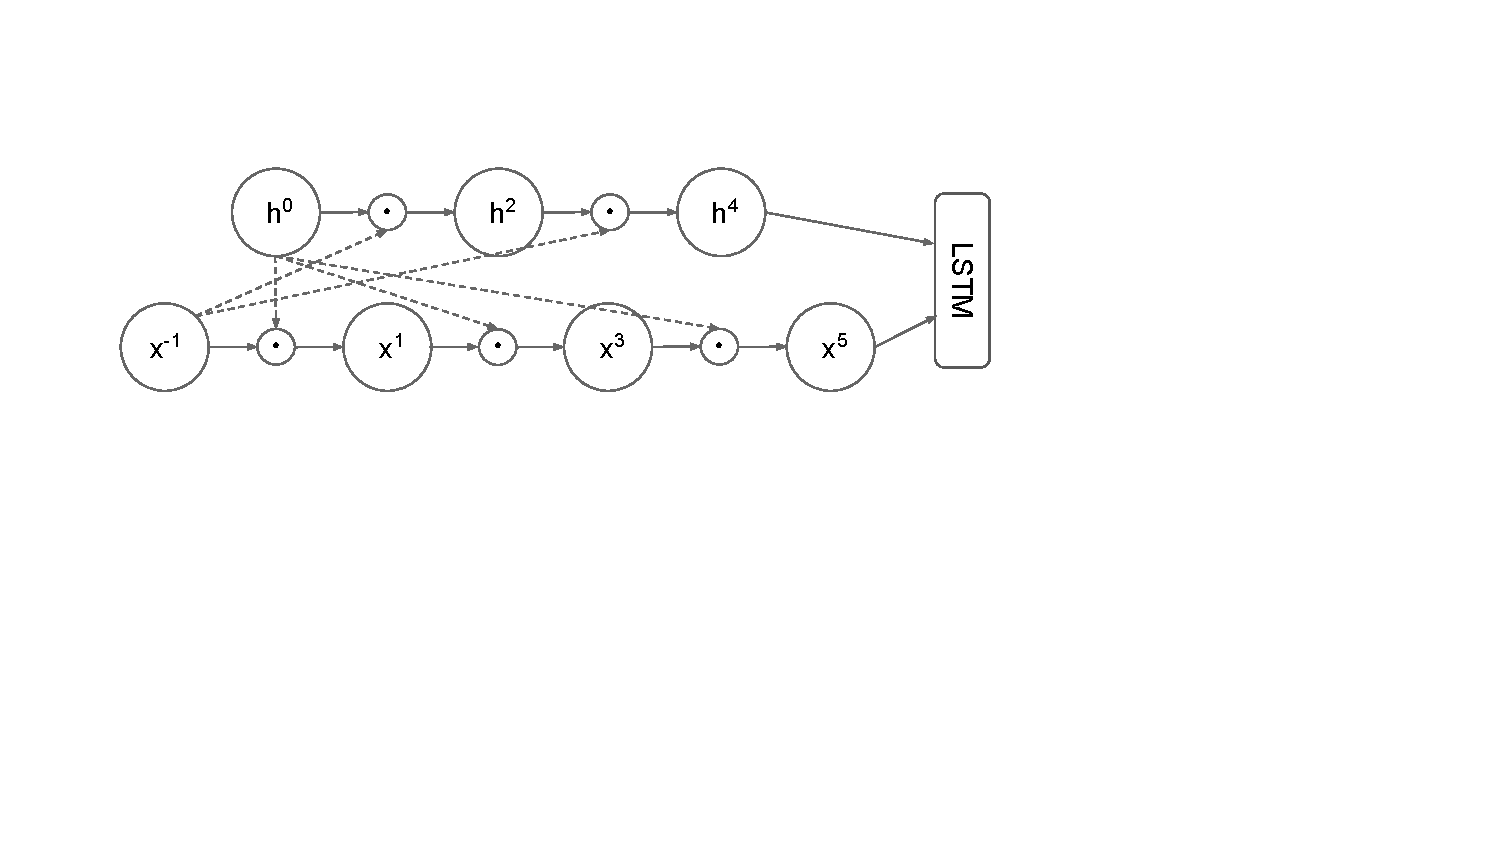
\includegraphics[scale=0.7,trim={1.8cm 7.5cm 8.3cm 2.5cm},clip]
                  {mogrifier/figure/mogrifier-no-zigzag.pdf}
  \caption[No-zigzag Mogrifier for the ablation study.]{No-zigzag Mogrifier for the ablation study, whose gating is always based on the original inputs.}
  \label{fig:mogrifier-no-zigzag}
\end{figure}
%
That is, in \eqref{eq:mogrify} the updates are changed to these no-zigzag variants:
\begin{align*}
  \vx^i &= 2\sigma\bigl(\mQ^{i}\vhprev\bigr) \odot \vx^{i-2} &
  \text{for odd i} \in [1..r],\\
  \vhprev^i &= 2\sigma\bigl(\mR^{i}\vx\bigr) \odot \vhprev^{i-2}
  & \text{for even i} \in [1..r].
\end{align*}
In our experiments, the no-zigzag variant underperformed the baseline
Mogrifier by a small but significant margin, and was on par with the
$r=2$ model in \Cref{fig:ppl-vs-rounds} suggesting that the
Mogrifier's iterative refinement scheme does more than simply widen
the range of possible gating values of $\vx$ and $\vhprev$ to $(0,
2^{\lceil r/2 \rceil})$ and $(0, 2^{\lfloor r/2 \rfloor})$,
respectively.

\begin{figure}
\begin{minipage}{0.5\linewidth}
  \begin{tikzpicture}
    \begin{axis}[width=1.05\linewidth, height=3.8cm,
        x label style={at={(axis description cs:0.5,-0.15)},anchor=north},
        y label style={at={(axis description cs:-0.11,.5)},rotate=0,
                       anchor=south},
        xlabel=$r$ rounds,
        ylabel=PPL,
        cycle list name=acycle]
	\addplot+ coordinates {
	  (0, 57.5) (1, 56.4) (2, 55.5)
          (3, 54.82) (4, 54.1) (5, 54.3) (6, 54.6)
	};
    \end{axis}
  \end{tikzpicture}
\captionof{figure}{Perplexity vs the number of rounds $r$ in the \ptb ablation
  study.}
\label{fig:ppl-vs-rounds}
\end{minipage}
\hfill
\begin{minipage}{0.46\linewidth}
\setlength\tabcolsep{36pt}
\begin{tabularx}{\textwidth}{@{}lr@{}}
  \midrule
  Mogrifier      & \nlltoppl{3.99163}  \\
  Full rank $Q^i,P^i$ & \nlltoppl{3.99947} \\
  No zigzag      & \nlltoppl{4.00647} \\
  LSTM           & \nlltoppl{4.051} \\
  mLSTM          & \nlltoppl{4.05750} \\
  \midrule
\end{tabularx}
\vspace{0.6\baselineskip}
\captionof{table}{PTB ablation study
  validation perplexities with 24M parameters.}
\label{tab:ablation}
\end{minipage}
\end{figure}

\subsection{Comparison to the mLSTM}
\label{seq:comparison-to-the-mlstm}

The Multiplicative LSTM \citep{DBLP:journals/corr/KrauseLMR16}, or
mLSTM for short, is closest to our model in the literature.
%
Formulating it as
\begin{gather*}
\mLSTM\bigl(\vx, \vcprev, \vhprev\bigr) = \LSTM\bigl(\vx, \vcprev, \vhprev^m\bigr)\\
\vhprev^m = \bigl(\mW^{mx} \vx\bigr) \odot \bigl(\mW^{mh} \vhprev\bigr),
\end{gather*}
%
the differences are readily apparent.
%
First, the mLSTM allows for multiplicative interaction between $\vx$
and $\vhprev$, but it only overrides $\vhprev$, while in the Mogrifier
the interaction is two-way, which --~as the ablation study showed~--
is important.
%
Second, the mLSTM can change not only the magnitude but also the sign
of values in $\vhprev$, something with which we experimented in the
Mogrifier, but could not get to work.
%
Furthermore, in the definition of $\vhprev^m$, the unsquashed
linearities and their elementwise product make the mLSTM more
sensitive to initialization and unstable during optimization.

On the \enwik dataset, we greatly improved on the published results of
the mLSTM \citep{DBLP:journals/corr/KrauseLMR16}.
%
In fact, even our LSTM baseline outperformed the mLSTM by 0.03 bpc.
%
We also conducted experiments on \ptb based on our reimplementation of
the mLSTM following the same methodology as the ablation study and
found that the mLSTM did not improve on the LSTM (see
\Cref{tab:ablation}).

\cite{DBLP:journals/corr/KrauseLMR16} posit and verify the recovery
hypothesis that says that having just suffered a large loss, the loss
on the next time step will be smaller on average for the mLSTM than
for the LSTM.
%
This was found not to be the case for the Mogrifier.
%
Neither did we observe a significant change in the gap between the
LSTM and the Mogrifier in the tied and untied embeddings settings,
which would be expected if recovery was affected by $\vx$ and
$\vhprev$ being in different domains.

\subsection{The Reverse Copy Task}

Our original motivation for the Mogrifier was to allow the context to
amplify salient and attenuate nuisance features in the input
embeddings.
%
We conduct a simple experiment to support this point of view.
%
Consider the reverse copy task where the network reads an input
sequence of tokens and a marker token after which it has to repeat the
input in reverse order.
%
In this simple sequence-to-sequence learning
\citep{sutskever2014sequence} setup, the reversal is intended to avoid
the minimal time lag problem \citep{hochreiter1997lstm}, which is not
our focus here.

The experimental setup is as follows.
%
For the training set, we generate \num{500000} examples by uniformly
sampling a given number of tokens from a vocabulary of size
\num{1000}.
%
The validation and test sets are constructed similarly, and contain
\num{10000} examples.
%
The model consists of an independent, unidirectional encoder and a
decoder, whose total number of parameters is \num{10} million.
%
The decoder is initialized from the last state of the encoder.
%
Since overfitting is not an issue here, no dropout is necessary, and
we only tune the learning rate, the l2 penalty, and the embedding size for
the LSTM.
%
For the Mogrifier, the number of rounds $r$ and the rank $k$ of the
low-rank approximation are also tuned.

\begin{figure}[!t]
  \begin{subfigure}{0.49\linewidth}
  \begin{tikzpicture}
    \begin{axis}[width=1.1 \linewidth, height=4.5cm,
        legend pos = north west,
        legend style={font=\footnotesize},
        x label style={at={(axis description cs:0.5,-0.15)},anchor=north},
        y label style={at={(axis description cs:-0.1,.5)},rotate=0,
                       anchor=south},
        xlabel=sequence length,
        ylabel=XE,
        cycle list name=acycle]
	\addplot+ coordinates {
		(50, 0.00020) (100, 0.05715) (150, 0.62399) (200, 1.80348)
	};
	\addplot+ coordinates {
		(50, 0.00038) (100, 0.07821) (150, 0.27998) (200, 1.39342)
	};
    \legend{$LSTM$,$Mogrifier$}
    \end{axis}
  \end{tikzpicture}
  \caption{10M parameters with vocabulary size 1k.}
  \label{fig:copy-10m-results}
  \end{subfigure}
  \hfill
  \begin{subfigure}{0.47\linewidth}
  \begin{tikzpicture}
    \begin{axis}[width=1.1\linewidth, height=4.5cm,
        legend pos = north west,
        legend style={font=\footnotesize},
        x label style={at={(axis description cs:0.5,-0.15)},anchor=north},
        y label style={at={(axis description cs:-0.1,.5)},rotate=0,
                       anchor=south},
        xlabel=sequence length,
        ylabel=XE,
        cycle list name=acycle]
	\addplot+ coordinates {
		(50, 0.14) (100, 0.25) (150, 1.49) (200, 3.99)
	};
	\addplot+ coordinates {
		(50, 0.03) (100, 0.13) (150, 0.29) (200, 1.03)
	};
    \legend{$LSTM$,$Mogrifier$}
    \end{axis}
  \end{tikzpicture}
  \caption{24M parameters with vocabulary size 10k.}
  \label{fig:copy-24m-results}
  \end{subfigure}
  \caption[Cross-entropy vs sequence length in the reverse copy
    task.]{Cross-entropy vs sequence length in the reverse copy
    task with i.i.d.\ tokens. Lower is better. The Mogrifier is better
    than the LSTM even in this synthetic task with no resemblance to
    natural language.}
\end{figure}

We compare the case where both the encoder and decoder are LSTMs to
where both are Mogrifiers.
%
\Cref{fig:copy-10m-results} shows that, for sequences of length
50 and 100, both models can solve the task perfectly.
%
At higher lengths though, the Mogrifier has a considerable advantage.
%
Examining the best hyperparameter settings found, the embedding/hidden
sizes for the LSTM and Mogrifier are 498/787 vs 41/1054 at 150 steps,
and 493/790 vs 181/961 at 200 steps.
%
Clearly, the Mogrifier was able to work with a much smaller embedding
size than the LSTM, which is in line with our expectations for a model
with a more flexible interaction between the input and recurrent
state.
%
We also conducted experiments with a larger model and vocabulary size,
and found the effect even more pronounced (see
\Cref{fig:copy-24m-results}).

\subsection{What the Mogrifier is Not}

The results on the reverse copy task support our hypothesis that input
embeddings are enriched by the Mogrifier architecture, but that cannot
be the full explanation as the results of the ablation study indicate.
%
In the following, we consider a number of hypotheses about where the
advantage of the Mogrifier lies and the experiments that provide
evidence \emph{against} them.
\begin{itemize}
\renewcommand\labelitemi{\scriptsize\Lightning}
\item \emph{Hypothesis: the benefit is in scaling $\vx$ and
  $\vhprev$.} We verified that data dependency is a crucial feature by
  adding a learnable scaling factor to the LSTM inputs. We observed no
  improvement. Also, at extremely low-rank (less than 5) settings
  where the amount of information in its gating is small, the
  Mogrifier loses its advantage.
\item \emph{Hypothesis: the benefit is in making optimization easier.}
  We performed experiments with different optimizers (SGD, RMSProp),
  with intra-layer batch normalization and layer normalization on the
  LSTM gates. While we cannot rule out an effect on optimization
  difficulty, in all of these experiments the gap between the LSTM and
  the Mogrifier was the same.
\item \emph{Hypothesis: exact tying of embeddings is too constraining,
  the benefit is in making this relationship less strict.} Experiments
  conducted with untied embeddings and character-based models
  demonstrate improvements of similar magnitude.
\item \emph{Hypothesis: the benefit is in the low-rank factorization
  of $\mQ^{i}, \mR^{i}$ implicitly imposing structure on the LSTM
  weight matrices.} We observed that the full-rank Mogrifier also
  performed better than the plain LSTM. We conducted additional
  experiments where the LSTM's gate matrices were factorized and
  observed no improvement.
\item \emph{Hypothesis: the benefit comes from better performance on
  rare words.} The observed advantage on character-based modelling is
  harder to explain based on frequency. Also, in the reverse copy
  experiments, a large number of tokens were sampled uniformly, so
  there were no rare words to speak of.
\item \emph{Hypothesis: the benefit is specific to the English
  language.} The improvements observed on the Finnish dataset and the
  reverse copy experiments, which did not feature natural language at
  all, directly contradict this hypothesis.
\item \emph{Hypothesis: the benefit is in handling long-range
  dependencies better.} Experiments in the episodic setting (i.e.
  sentence-level language modelling) exhibited the same gap as the
  non-episodic ones.
\item \emph{Hypothesis: the scaling up of inputs saturates the
  downstream LSTM gates.} The idea here is that saturated gates may
  make states more stable over time. We observed the opposite: the
  means of the standard LSTM gates in the Mogrifier were very close
  between the two models, but their variance was smaller in the
  Mogrifier.
\end{itemize}

\section{Conclusions}

\mglconclusion
Many advances in natural language processing have been based upon more
expressive models for how inputs interact with the context in which
they occur.
%
Recurrent networks, which have enjoyed a modicum of success, still
lack the generalization and systematicity ultimately required for
modelling language.
%
In this work, we proposed an extension to the venerable Long Short-Term
Memory in the form of mutual gating of the current input and the
previous output.
%
This mechanism affords the modelling of a richer space of interactions
between inputs and their context.
%
Equivalently, our model can be viewed as making the transition
function given by the LSTM context-dependent.
%
Experiments demonstrate markedly improved generalization on language
modelling in the range of 3--4 perplexity points on Penn Treebank and
\wikitexttwo, and 0.01--0.05 bpc on four character-based datasets.
%
With the Mogrifier LSTM, we establish a new state of the art on all
datasets with the exception of \enwik, where we close a large gap
between the LSTM and Transformer models.

Our original motivation for this work was that the context-free
representation of input tokens may be a bottleneck in language models,
and by conditioning the input embedding on the recurrent state some
benefit was indeed derived.
%
While it may be part of the explanation, this interpretation clearly
does not account for the improvements brought by conditioning the
recurrent state on the input and especially the benefits of mogrification on
character-level datasets.
%
Positioning our work on the Multiplicative RNN line of research offers
a more compelling perspective.

To give more credence to this interpretation, in the analysis we
highlighted a number of possible alternative explanations and ruled
them all out to varying degrees.
%
In particular, the connection to the mLSTM was found to be weaker than
expected as the Mogrifier does not exhibit improved recovery (see
\Cref{seq:comparison-to-the-mlstm}), and on \ptb the mLSTM
works only as well as the LSTM.
%
At the same time, the evidence against easier optimization is weak,
and the Mogrifier establishing some kind of sharing between otherwise
independent LSTM weight matrices is a distinct possibility.

Finally, note that as shown by \Cref{fig:mogrifier} and
\eqref{eq:mogrify}, the Mogrifier is a series of preprocessing
steps composed with the LSTM function, but other architectures, such
as Mogrifier GRU or Mogrifier Elman Network are possible.
%
We also leave investigations into other forms of parameterization of
context-dependent transitions for future work.

\mglsep

\chapter*{Appendices}

\begin{subappendices}

\section{Hyperparameter Tuning Ranges}
\label{sec:hyperparameter-tuning-ranges}

In all experiments, we tuned hyperparameters using Google Vizier
\citep{golovin2017google}.
%
The tuning ranges are listed in
\Cref{tab:hyperparameter-tuning-ranges}.
%
Obviously, \emph{mogrifier\_rounds} and \emph{mogrifier\_rank} are
tuned only for the Mogrifier.
%
If $input\_embedding\_ratio \geqslant 1$, then the input/output
embedding sizes and the hidden sizes are set to equal and the linear
projection from the cell output into the output embeddings space is
omitted.
%
Similarly, $mogrifier\_rank \leqslant 0$ is taken to mean full rank
$\mQ^{*}$, $\mR^{*}$ without factorization.
%
Since \enwik is a much larger dataset, we do not tune
\emph{input\_embedding\_ratio} and specify tighter tuning ranges for
dropout based on preliminary experiments (see
\Cref{tab:hyperparameter-tuning-ranges-enwik}).

Dynamic evaluation hyperparameters were tuned according to
\Cref{tab:hyperparameter-tuning-ranges-dyneval}.
%
The highest possible value for \emph{max\_time\_steps}, the BPTT
window size, was 20 for word, and 50 for character-level tasks.
%
The batch size for estimating the mean squared gradients over the
training data was set to 1024, gradient clipping was turned off, and
the l2 penalty was set to zero.

\begin{table}[tp]
  \caption{Hyperparameter tuning ranges for all tasks except
    \enwik.}
  \label{tab:hyperparameter-tuning-ranges}

  \centering
  \begin{tabular}{@{}lrrrr@{}}
    & Low & High & Spacing \\
    \midrule
    learning\_rate & 0.001 & 0.004 & log \\
    input\_embedding\_ratio & 0.0 & 2.0 & \\
    l2\_penalty & 5e-6 & 1e-3 & log \\
    input\_dropout & 0.0 & 0.9 & \\
    inter\_layer\_dropout & 0.0 & 0.95 & \\
    state\_dropout & 0.0 & 0.8 \\
    output\_dropout & 0.0 & 0.95 \\
    mogrifier\_rounds ($r$) & 0 & 6 \\
    mogrifier\_rank ($k$) & -20 & 100 \\
    \midrule
  \end{tabular}
\end{table}

\begin{table}[tp]
  \caption{Hyperparameter tuning ranges for \enwik.}
  \label{tab:hyperparameter-tuning-ranges-enwik}

  \centering
  \begin{tabular}{@{}lrrrr@{}}
    & Low & High & Spacing \\
    \midrule
    learning\_rate & 0.001 & 0.004 & log \\
    l2\_penalty & 5e-6 & 1e-3 & log \\
    input\_dropout & 0.0 & 0.2 & \\
    inter\_layer\_dropout & 0.0 & 0.2 & \\
    state\_dropout & 0.0 & 0.25 \\
    output\_dropout & 0.0 & 0.25 \\
    mogrifier\_rounds ($r$) & 0 & 6 \\
    mogrifier\_rank ($k$) & -20 & 100 \\
    \midrule
  \end{tabular}
\end{table}

\begin{table}[tp]
  \caption{Hyperparameter tuning ranges for dynamic evaluation.}
  \label{tab:hyperparameter-tuning-ranges-dyneval}

  \centering
  \begin{tabular}{@{}lrrrr@{}}
    & Low & High & Spacing \\
    \midrule
    max\_time\_steps & 1 & 20/50 & \\
    dyneval\_learning\_rate & 1e-6 & 1e-3 & log \\
    dyneval\_decay\_rate & 1e-6 & 1e-2 & log \\
    dyneval\_epsilon & 1e-8 & 1e-2 & log \\
    \midrule
  \end{tabular}
\end{table}

\section{Hyperparameter Sensitivity}
\label{sec:hyperparameter-sensitivity}

The parallel coordinate plots in \Cref{fig:lstm-sensitivity} and
\ref{fig:fm-sensitivity} give a rough idea about hyperparameter
sensitivity.
%
The red lines correspond to hyperparameter combinations closest to the
best solution found.
%
To find the closest combinations, we restricted the range for each
hyperparameter separately to about 15\% of its entire tuning range.
%
For both the LSTM and the Mogrifier, the results are at most 1.2
perplexity points off the best result, so our results are somewhat
insensitive to jitter in the hyperparameters.
%
Still, in this setup, grid search would require orders of magnitude
more trials to find comparable solutions.

On the other hand, the tuner does take advantage of the stochasticity
of training, and repeated runs with the same parameters may give
slightly worse results.
%
To gauge the extent of this effect, on \ptb we estimated the standard
deviation in reruns of the LSTM with the best hyperparameters to be
about 0.2 perplexity points, but the mean was about 0.7 perplexity
points off the result produced with the weights saved in best tuning
run.

\begin{figure}[tp]\centering
  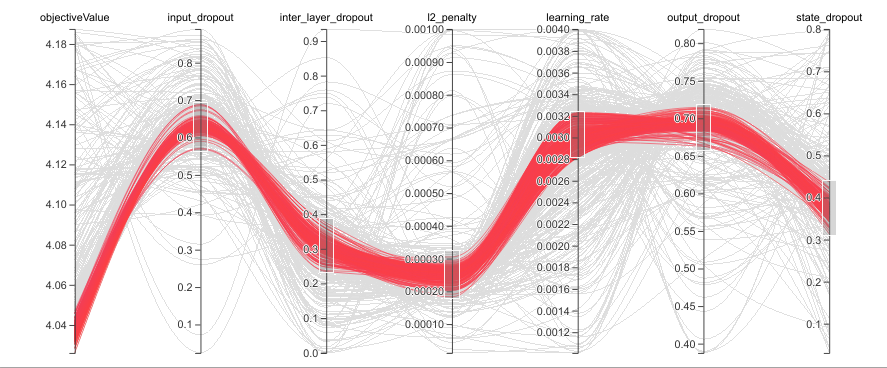
\includegraphics[width=0.98\textwidth,trim={0cm 0.1cm 0.0cm 0cm},clip]
                  {mogrifier/figure/ptb-24m-lstm-d2-sensitivity.png}
  \caption[LSTM hyperparameter sensitivity on PTB.]{Average
    per-word validation cross-entropies for hyperparameter
    combinations in the neighbourhood of the best solution for a
    2-layer LSTM with 24M weights on the Penn Treebank dataset.}
  \label{fig:lstm-sensitivity}
\end{figure}

\begin{figure}[tp]\centering
  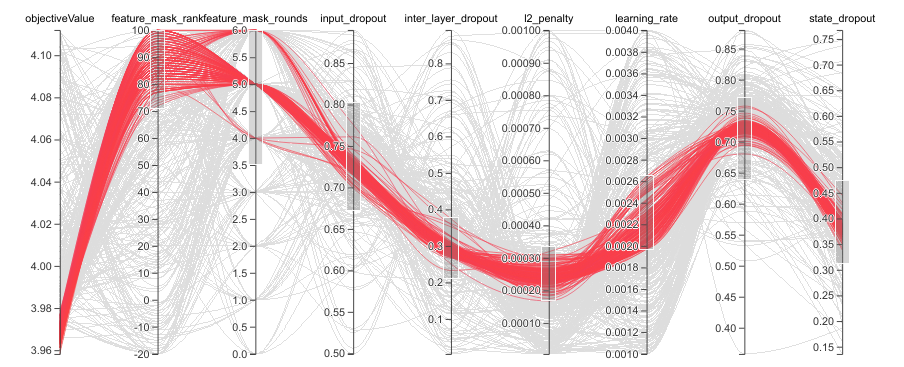
\includegraphics[width=0.98\textwidth,trim={0cm 0.1cm 0.0cm 0cm},clip]
                  {mogrifier/figure/ptb-24m-fm-d2-sensitivity.png}
  \caption[Mogrifier hyperparameter sensitivity on PTB.]{Average
    per-word validation cross-entropies for hyperparameter
    combinations in the neighbourhood of the best solution for a
    2-layer Mogrifier LSTM with 24M weights on the Penn Treebank
    dataset. \emph{feature\_mask\_rank} and
    \emph{feature\_mask\_rounds} are aliases for
    \emph{mogrifier\_rank} and \emph{mogrifier\_rounds}}.
  \label{fig:fm-sensitivity}
\end{figure}

\end{subappendices}
